% RRC2026_report.tex -- Power-based normalization of the Råda Rowing Challenge 2026 mixed relay
%
% Build:  python generate_figures.py      (figures + tables + numbers.tex, from the ergrace package)
%         pdflatex RRC2026_report.tex     (run twice for cross-references)
%
% All numbers marked with a macro (e.g. \MeanScore) are computed by generate_figures.py
% and read from figures/numbers.tex, so text, tables and figures cannot drift apart.

\documentclass[twocolumn, 10pt]{article}

% ── Encoding & fonts ─────────────────────────────────────────────────────────
\usepackage[utf8]{inputenc}
\usepackage[T1]{fontenc}
\usepackage{mathptmx}
\usepackage{microtype}

% ── Layout ───────────────────────────────────────────────────────────────────
\usepackage[a4paper, top=2.5cm, bottom=2.5cm, left=1.5cm, right=1.5cm,
            columnsep=0.7cm]{geometry}

% ── Math & units ─────────────────────────────────────────────────────────────
\usepackage{amsmath}
\usepackage{siunitx}
\sisetup{separate-uncertainty=true, per-mode=power, range-phrase=\text{--}}

% ── Tables & figures ─────────────────────────────────────────────────────────
\usepackage{booktabs}
\usepackage{graphicx}
\usepackage{caption}
\captionsetup{font=small, labelfont=bf}
\usepackage{pgfplots}
\pgfplotsset{compat=1.16}

% ── Layout helpers & sections ────────────────────────────────────────────────
\usepackage{parskip}
\setlength{\parskip}{4pt}
\usepackage{titlesec}
\renewcommand{\thesection}{\Roman{section}}
\titleformat{\section}{\normalfont\bfseries\centering}{\thesection.}{0.5em}{\MakeUppercase}
\titleformat{\subsection}{\normalfont\itshape}{\thesubsection.}{0.5em}{}
\renewcommand{\abstractname}{}

\usepackage{xurl}
\usepackage{hyperref}
\hypersetup{colorlinks=true, linkcolor=black, citecolor=black, urlcolor=blue}

% ── Notation ─────────────────────────────────────────────────────────────────
\newcommand{\Pref}{P^{\mathrm{ref}}}
\newcommand{\Dref}{D^{\mathrm{ref}}}
% generated by generate_figures.py -- do not edit
\newcommand{\PmTwoK}{597}
\newcommand{\PfTwoK}{405}
\newcommand{\RatioTwoK}{1.48}
\newcommand{\SpeedRatioTwoK}{1.139}
\newcommand{\MeanDist}{8.60}
\newcommand{\StdDist}{0.76}
\newcommand{\CvDist}{8.8}
\newcommand{\MeanScore}{0.65}
\newcommand{\MeanSpeedScore}{0.858}
\newcommand{\MinScore}{0.34}
\newcommand{\MaxScore}{0.80}
\newcommand{\TieMargin}{0.5}
\newcommand{\FirstTeam}{Chalmers 1}
\newcommand{\SecondTeam}{CTH-GU}
\newcommand{\FirstScore}{0.8033}
\newcommand{\SecondScore}{0.8031}
\newcommand{\ScoreGap}{$1.2\times10^{-4}$}
\newcommand{\MaxBiasTwoK}{1.3}
\newcommand{\OldFirst}{CTH-GU}
\newcommand{\OldSecond}{Chalmers 1}
\newcommand{\TopSplit}{1:37.1}
\newcommand{\TopRefSplit}{1:30.3}
\newcommand{\TopSpeedDeficit}{7}
\newcommand{\TopPowerDeficit}{20}
\newcommand{\RatioFive}{1.77}
\newcommand{\MaxBiasFive}{2.8}
\newcommand{\RatioOneK}{1.72}
\newcommand{\MaxBiasOneK}{2.5}
\newcommand{\RatioFiveK}{1.44}
\newcommand{\MaxBiasFiveK}{1.1}

\makeatletter\newcommand{\tableinput}[1]{\@@input #1 }\makeatother % \input that works inside tabular

% ──────────────────────────────────────────────────────────────────────────────
\title{\textbf{Power-Based Normalization of Team Performance\\ in Mixed Indoor Rowing Relays}}

\author{Lukas Johannes Splitthoff\textsuperscript{1,2},
        Johan Lysemark\textsuperscript{2},
        Oscar Gyllensten\textsuperscript{2}\\[4pt]
        \small\textsuperscript{1}Department of Microtechnology and Nanoscience (MC2),
        Chalmers University of Technology,\\
        \small Kemiv{\"a}gen 9, SE-412 58 G{\"o}teborg, Sweden\\
        \small\textsuperscript{2}M{\"o}lndals Roddklubb, R{\aa}dav{\"a}gen 38, SE-431 36 M{\"o}lndal, Sweden}

\date{7 March 2026 (revised 24 September 2026)}

% ══════════════════════════════════════════════════════════════════════════════
\begin{document}

\twocolumn[
  \maketitle
  \begin{abstract}
  \noindent
  We normalize the results of a mixed-gender indoor-rowing relay, the
  R{\aa}da Rowing Challenge 2026, in which ten five-person teams of different
  gender composition shared one ergometer each for 30 minutes.
  Each team is scored by the fraction $\sigma$ of reference power that its
  rowers sustained, where the reference is set by world indoor-rowing records.
  Because relay members row one after another, their \emph{distances} add,
  not their powers; the team reference matching the measured distance is
  therefore the power mean with exponent $1/3$ of the individual reference
  powers, and the score reduces to $\sigma=(D/\Dref)^3$, independent of the
  monitor's power--speed constant.
  Comparing the power at the team's mean speed with the arithmetic mean of
  reference powers, the intuitive alternative, is biased against mixed teams
  by up to \MaxBiasTwoK\,\% and is enough to swap the top two places.
  Expressing the score in power rather than speed does not change the order,
  but it reports what the athletes actually produce: a 7\,\% speed deficit is
  a 20\,\% power deficit.
  The ranking is instead sensitive to the choice of reference distance,
  which we quantify.
  With \SI{2000}{m} records as reference, the two leading teams finish in a
  dead heat, \TieMargin\,m apart.
  \end{abstract}
  \vspace{1em}
]

% ══════════════════════════════════════════════════════════════════════════════
\section{Introduction}

The R{\aa}da Rowing Challenge (RRC) is an indoor rowing competition organized
by M{\"o}lndals Roddklubb~\cite{MRKhomepage}, held annually at R{\aa}daRum in
M{\"o}lnlycke, Sweden.
The 2026 edition took place on 7~March 2026 and included individual events as
well as a 30-minute mixed relay~\cite{MRKweb2026}.
In the relay, each team of five rowers shares \emph{one} Concept2 RowErg,
taking turns on the machine; the team's result is the total distance shown by
the monitor after \SI{30}{min}.

Ten teams entered: Chalmers Roddklubb (two teams), J{\"o}nk{\"o}pings
Rodds{\"a}llskap (two teams), Halmstads Roddklubb, M{\"o}lndals Roddklubb
(two teams), G{\"o}teborgs Roddklubb, R{\aa}da Crew, and CTH-GU.
Compositions ranged from all-female (G{\"o}teborgs Roddklubb) to four men and
one woman (Chalmers Roddklubb -- Team~2).
Because men and women differ systematically in ergometer output, raw distance
favours teams with more men.

We develop a composition-aware score in four steps:
the ergometer's power--speed relation (Sec.~\ref{sec:formula}),
reference performances and the gender gap (Sec.~\ref{sec:records}),
a physical model of the relay that fixes how individual references combine
(Sec.~\ref{sec:normalization}), and
the results with a sensitivity analysis (Sec.~\ref{sec:results}).

% ══════════════════════════════════════════════════════════════════════════════
\section{The Ergometer Power Formula}
\label{sec:formula}

The Concept2 monitor derives a speed $v$ from the angular deceleration of the
air-braked flywheel; $v$ is the speed of a virtual boat, not the handle speed.
It converts speed to power with the fixed relation~\cite{Concept2manual}
\begin{equation}
  P = c\,v^{3}, \qquad c = \SI{2.8}{\watt\second\cubed\per\metre\cubed}
  = \SI{2.8}{\kilo\gram\per\metre}.
  \label{eq:power}
\end{equation}
The cubic law mirrors a boat moving against hydrodynamic drag
$F\propto v^{2}$, for which the propulsive power is $P=Fv\propto v^{3}$;
$c$ is a conversion constant defined by Concept2 rather than a measured
property of an individual machine.
For a distance $d$ rowed in time $t$, the average speed is $v=d/t$; in terms of
the 500-metre split $t_{500}=\SI{500}{m}/v$,
\begin{equation}
  P = c\left(\frac{\SI{500}{m}}{t_{500}}\right)^{\!3}.
  \label{eq:power_split}
\end{equation}
For example, $t_{500}=\SI{120}{s}$ (2:00) gives \SI{202.5}{W}, and the men's
\SI{2000}{m} world record (\SI{334.7}{s}, $t_{500}=\SI{83.7}{s}$) gives
\SI{\PmTwoK}{W}.
Figure~\ref{fig:power_curve} shows the strong nonlinearity.

Two properties matter below.
First, the displayed power is computed from speed; it is not measured at the
handle, and force-sensor studies find it differs from the mechanical power
delivered by the rower~\cite{Boyas2006}.
Our method uses only distances and times, so it is unaffected.
Second, $c$ drops out of every score we define (Sec.~\ref{sec:normalization}),
so its precise value is irrelevant for the ranking.

\begin{figure}[t]
  \centering
  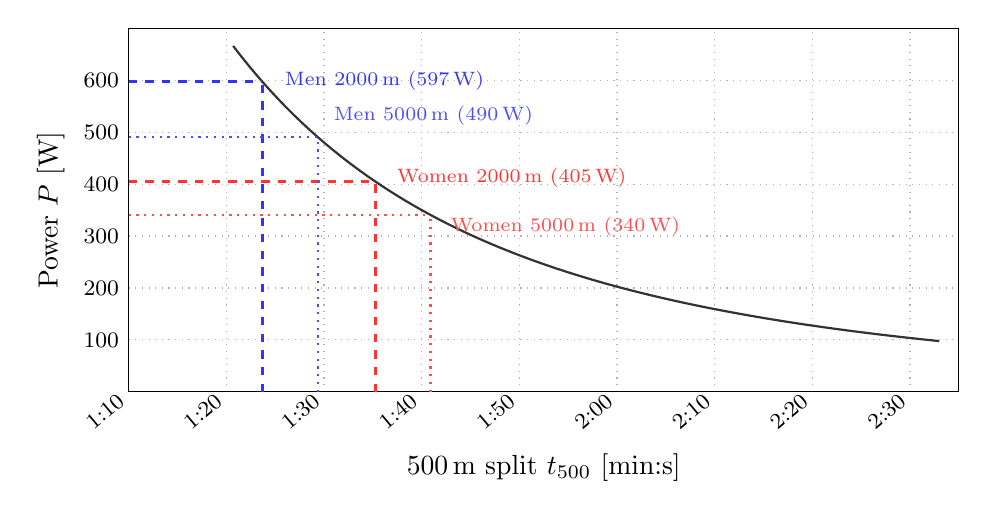
\begin{tikzpicture}
    \begin{axis}[
        width=\columnwidth, height=6.2cm,
        xlabel={500\,m split $t_{500}$ [min:s]},
        ylabel={Power $P$ [W]},
        xmin=70, xmax=155, ymin=0, ymax=700,
        ytick={100,200,300,400,500,600},
        xtick={70,80,90,100,110,120,130,140,150},
        xticklabels={1:10,1:20,1:30,1:40,1:50,2:00,2:10,2:20,2:30},
        x tick label style={rotate=40, anchor=east, font=\footnotesize},
        yticklabel style={font=\footnotesize},
        grid=major, grid style={dotted, gray!60},
        tick style={draw=none}, clip=false,
      ]
      \addplot[thick, black!80, domain=80.7:153, samples=300] {2.8*(500/x)^3};
      % 2000 m world records (reference used in this study)
      \addplot[dashed, blue!80, very thick] coordinates {(83.7,0)(83.7,597)};
      \addplot[dashed, blue!80, very thick] coordinates {(70,597)(83.7,597)};
      \node[font=\scriptsize, blue!80, anchor=west] at (axis cs:85,600) {Men 2000\,m (597\,W)};
      \addplot[dashed, red!80, very thick] coordinates {(95.3,0)(95.3,405)};
      \addplot[dashed, red!80, very thick] coordinates {(70,405)(95.3,405)};
      \node[font=\scriptsize, red!80, anchor=west] at (axis cs:96.5,412) {Women 2000\,m (405\,W)};
      % 5000 m world records
      \addplot[dotted, blue!70, thick] coordinates {(89.4,0)(89.4,490)};
      \addplot[dotted, blue!70, thick] coordinates {(70,490)(89.4,490)};
      \node[font=\scriptsize, blue!70, anchor=south west] at (axis cs:90,494) {Men 5000\,m (490\,W)};
      \addplot[dotted, red!70, thick] coordinates {(100.9,0)(100.9,340)};
      \addplot[dotted, red!70, thick] coordinates {(70,340)(100.9,340)};
      \node[font=\scriptsize, red!70, anchor=west] at (axis cs:102,318) {Women 5000\,m (340\,W)};
    \end{axis}
  \end{tikzpicture}
  \caption{Ergometer power versus 500\,m split, Eq.~\eqref{eq:power_split}.
    Dashed: \SI{2000}{m} world records (reference used in this study).
    Dotted: \SI{5000}{m} world records.}
  \label{fig:power_curve}
\end{figure}

% ══════════════════════════════════════════════════════════════════════════════
\section{Reference Performance}
\label{sec:records}

\subsection{Indoor rowing records}

Table~\ref{tab:records} lists reference performances on the Concept2 RowErg.
The \SIlist{500;2000;5000}{m} entries are world records from the Concept2
records database~\cite{Concept2records}; the \SI{1000}{m} entries are
event-winning times from the 2026 World Rowing Virtual Indoor Championships
(WRVIC~2026)~\cite{WorldRowingWRVIC2026} and are not necessarily records.

\begin{table}[ht]
  \centering
  \caption{Reference performances (Concept2 RowErg, open category) and the
           corresponding power, Eq.~\eqref{eq:power_split}.}
  \label{tab:records}
  \setlength{\tabcolsep}{4pt}
  \begin{tabular}{@{}llcrl@{}}
    \toprule
    Dist. & Gender & Time [min:s] & $P$ [W] & Athlete (year)\\
    \midrule
    500\,m  & Men   & 1:09.8  & 1029 & P.\ Clapp (2024)    \\
    500\,m  & Women & 1:24.5  &  580 & O.\ Buryak (2017)   \\
    1000\,m & Men   & 2:38.0  &  710 & A.\ Panizza (2026)  \\
    1000\,m & Women & 3:09.4  &  412 & A.\ Ader (2026)     \\
    2000\,m & Men   & 5:34.7  &  597 & O.\ Zeidler (2026)  \\
    2000\,m & Women & 6:21.1  &  405 & B.\ Mooney (2021)   \\
    5000\,m & Men   & 14:53.9 &  490 & T.\ George (2022)   \\
    5000\,m & Women & 16:49.4 &  340 & G.\ Rowe (2026)     \\
    \bottomrule
  \end{tabular}
\end{table}

\subsection{The gender gap in speed and in power}

At \SI{2000}{m} the men's record is faster by a factor
$v_m/v_f=381.1/334.7=\SpeedRatioTwoK$, i.e.\ 14\,\% in speed, but by
$P_m/P_f=(v_m/v_f)^3=\RatioTwoK$ in power.
The cubic law turns a moderate speed advantage into a large difference in
produced power.
The ratio also depends on distance
(Fig.~\ref{fig:reference}a): $P_m/P_f=\RatioFive$, \RatioOneK, \RatioTwoK\
and \RatioFiveK\ at \SIlist{500;1000;2000;5000}{m}.
The men's advantage is largest in short, predominantly anaerobic efforts.
The \SI{1000}{m} values are race results rather than records and should be
read with that caveat; the trend is carried by the three record distances.

As shown in Sec.~\ref{sec:normalization}, a normalized \emph{ranking}
depends on the references only through this ratio: multiplying both reference
powers by a common factor rescales every score but leaves the order unchanged.
Absolute record levels are therefore irrelevant for the ranking; the
choice of reference distance is not.

\subsection{Choice of reference distance}
\label{sec:refdistance}

Each relay member rows about \SI{6}{min} in total, which matches a
\SI{2000}{m} effort in duration, and covers about \SI{1.7}{km}, close to
\SI{2000}{m} in distance.
The work is, however, split into short bouts: teams typically swap about every
\SI{30}{s}, so each rower performs roughly a dozen short, hard bouts with
recovery in between.
Short bouts with recovery typically allow a higher power than one
continuous \SI{2000}{m} effort, and draw more on the anaerobic capacity that
dominates the shorter events, where the gender gap is larger.
We therefore expect the appropriate ratio to lie at or above the
\SI{2000}{m} value.
There is no unique correct reference distance.
We adopt the \SI{2000}{m} records as the primary reference, the standard
benchmark in rowing, and report the ranking for all four distances in
Sec.~\ref{sec:sensitivity}.

% ══════════════════════════════════════════════════════════════════════════════
\section{Normalization}
\label{sec:normalization}

\subsection{Relay model: distances add}

Team $k$ has $n$ rowers, $n_m$ men and $n_f$ women.
Rower $i$ rows for a total time $\tau_i$ at average speed $v_i$, with
$\sum_i\tau_i=T=\SI{1800}{s}$.
Because the rowers take turns on one machine, the monitor accumulates their
distances:
\begin{equation}
  D_k = \sum_{i=1}^{n} v_i\,\tau_i .
  \label{eq:relay}
\end{equation}
Powers do not add in a relay; only one rower produces power at any time.
We assume equal shares, $\tau_i=T/n$;
then $D_k/T=\bar v_k$ is the mean of the rowers' speeds.

\subsection{Uniform-effort hypothesis and the power score}

Let $P_i\in\{P_m,P_f\}$ be the reference power of rower $i$ and
$v_i^{\mathrm{ref}}=(P_i/c)^{1/3}$ the corresponding speed.
The fair question is: what fraction $\sigma_k$ of their reference power did
the rowers of team $k$ sustain?
If every rower holds the same fraction, $P=\sigma_k P_i$, then by
Eq.~\eqref{eq:power} each rows at $v_i=\sigma_k^{1/3}v_i^{\mathrm{ref}}$ and
Eq.~\eqref{eq:relay} gives
\begin{equation}
  D_k = \sigma_k^{1/3}\,\Dref_k, \qquad
  \Dref_k = \frac{T}{n}\sum_{i=1}^{n} v_i^{\mathrm{ref}},
  \label{eq:dref}
\end{equation}
where $\Dref_k$ is the distance a composition-matched team rowing exactly
at reference would cover.
Solving for $\sigma_k$ yields the \emph{power score}
\begin{equation}
  \boxed{\;\sigma_k = \left(\frac{D_k}{\Dref_k}\right)^{\!3}
        = \frac{P_k^{\mathrm{team}}}{\Pref_k}\;}
  \label{eq:score}
\end{equation}
with the power at the team's mean speed and its reference
\begin{align}
  P_k^{\mathrm{team}} &= c\left(\frac{D_k}{T}\right)^{\!3}, \label{eq:team_power}\\
  \Pref_k &= c\,\bigl(\bar v_k^{\mathrm{ref}}\bigr)^{3}
            = \Biggl[\frac{1}{n}\sum_{i=1}^{n}P_i^{1/3}\Biggr]^{3}.
  \label{eq:pref}
\end{align}
$\Pref_k$ is the power mean with exponent $1/3$ of the individual reference
powers: it equals $P_f$ for an all-female and $P_m$ for an all-male team
and increases monotonically with $n_m$.

Units are consistent throughout: $D_k$ and $\Dref_k$ are in metres, $\sigma_k$
is dimensionless, and $P^{\mathrm{team}}_k$ and $\Pref_k$ are in watts.
Writing the references as distances $d$ rowed in times $t_i$, so that
$v_i^{\mathrm{ref}}=d/t_i$, gives
$\sigma_k=\bigl[D_k\big/\bigl(\tfrac{T}{n}\sum_i d/t_i\bigr)\bigr]^3$.
Only distances and times enter; the constant $c$ cancels exactly.

The \emph{speed score} $s_k=D_k/\Dref_k$ is the same information on a
different scale, $\sigma_k=s_k^3$.
Both give identical rankings.

\subsection{Why score in power}

The ranking does not depend on whether the score is expressed in power or in
speed, so the case for power is not that it reorders teams.
It rests on three points.

\emph{(i) Power is the athlete's output.}
Power is the rate at which the rower does work on the machine, and the
reference records are power levels that athletes sustained.
Under the uniform-effort hypothesis every rower of team $k$ produced
$\sigma_kP_i$, so $\sigma_k=0.8$ means that the rowers sustained 80\,\% of
their reference power.
The speed score compresses this: to first order
$1-\sigma_k\approx3(1-s_k)$, and still by a factor 2--2.5 for the deficits in
this field.
A team 7\,\% slower than reference produced 20\,\% less power.
Speed understates how far teams are from the reference, and how different
they are from each other.

\emph{(ii) Power makes the combination rule explicit.}
Under the hypothesis, the rowers' mean \emph{produced} power is
$\sigma_k\langle P\rangle_k$ with $\langle P\rangle_k=(n_mP_m+n_fP_f)/n$, so
$\sigma_k$ is also the ratio of produced to reference mean power.
A relay monitor, however, does not record the mean produced power; it records
$D_k$, i.e.\ the mean \emph{speed}.
The power belonging to that observable is $P^{\mathrm{team}}_k=c\,\bar v_k^3$,
the power at the team's mean speed, and its matching reference is the power
at the reference team's mean speed, $\Pref_k$ of Eq.~\eqref{eq:pref}.
In a crew boat the situation is reversed: the rowers pull
\emph{simultaneously}, the observable boat speed is set by the sum of their
powers, and the arithmetic mean of seat powers is the matching reference.
Which mean is correct is decided by what the measurement records: summed
power for crews, summed distance for relays.

\emph{(iii) Mixing the two is biased.}
Dividing $P^{\mathrm{team}}_k$, the power at the team's mean speed, by the
arithmetic mean $\langle P\rangle_k$ compares two different quantities.
By the power-mean inequality $\Pref_k\le\langle P\rangle_k$, with equality only
for single-gender teams, so a mixed team rowing exactly at reference would
score below one.
The bias grows with the gender gap: at most \MaxBiasTwoK\,\% at
\SI{2000}{m} and \MaxBiasFive\,\% at \SI{500}{m}, largest for 2M/3F
(Fig.~\ref{fig:reference}b).
This is small, but not negligible here: with the mixed comparison the order of
the top two teams reverses (\OldFirst\ ahead of \OldSecond).

\subsection{Assumptions}

(a)~Equal shares of time per rower.
Individual rowing times were not recorded; a team that gave its fastest rowers
more time would gain relative to the reference.
(b)~Uniform effort: all rowers of a team at the same fraction of their
reference.
If instead every rower held the same fraction of reference \emph{speed}, the
score would be $s_k$, and $\sigma_k=s_k^3$ again gives the same ranking.
(c)~Changeovers: the flywheel coasts while rowers swap, and the monitor keeps
counting, so part of $T$ is not rowed by anyone.
The effect depends on the number and speed of changeovers.
It is similar for all teams but not modelled; it is contained in $D_k$.
(d)~All teams row on Concept2 RowErgs with the same monitor conversion; $c$
cancels in any case.
(e)~Reference powers are computed from the average speed of the record
efforts, $v=d/t$.
Records are not rowed at perfectly constant pace, but only these speeds enter
the score.

\begin{figure*}[t]
  \centering
  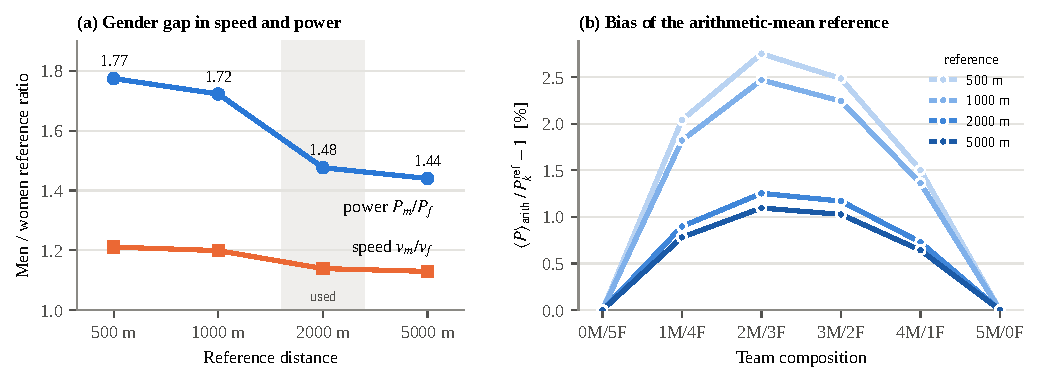
\includegraphics[width=0.9\textwidth]{figures/reference.pdf}
  \caption{(a)~Ratio of men's to women's reference speed (squares) and power
    (circles) versus reference distance, Table~\ref{tab:records}.
    The power ratio is the cube of the speed ratio.
    (b)~Relative overestimate of the team reference by the arithmetic mean of
    reference powers compared with the correct power mean $\Pref_k$,
    Eq.~\eqref{eq:pref}, for all compositions of a five-person team.
    Single-gender teams are unaffected; mixed teams are penalized, more so for
    shorter reference distances.}
  \label{fig:reference}
\end{figure*}

% ══════════════════════════════════════════════════════════════════════════════
\section{Results}
\label{sec:results}

\subsection{Normalized ranking}

With the \SI{2000}{m} records, $P_m=\SI{\PmTwoK}{W}$ and
$P_f=\SI{\PfTwoK}{W}$.
Table~\ref{tab:results} and Fig.~\ref{fig:results}a give the result.

The mean team distance was \SI{\MeanDist \pm \StdDist}{km} (mean $\pm$
sample standard deviation, coefficient of variation \CvDist\,\%).
The mean power score was \MeanScore: on average, the rowers sustained
about two thirds of world-record power for their composition, at a mean
speed score of \MeanSpeedScore.
Scores span \MinScore--\MaxScore.
All are below one, as expected for a record-based reference.

\emph{Dead heat for first place.}
\FirstTeam\ ($\sigma=\FirstScore$) and \SecondTeam\ ($\sigma=\SecondScore$)
are separated by \ScoreGap.
\SecondTeam\ would have needed only \TieMargin\,m more, out of
\SI{9.5}{km}, to draw level.
This is below the monitor's \SI{1}{m} resolution, so the two teams share
first place.

\emph{Composition matters.}
G{\"o}teborgs Roddklubb, the only all-female team, covered the seventh-longest
distance but ranks third.
Chalmers Roddklubb -- Team~2 (4M/1F) covered the third-longest distance but
ranks seventh, because four men set a reference of \SI{555}{W}.

\emph{Scale.}
\FirstTeam\ averaged \TopSplit\ per \SI{500}{m} against a reference
pace of \TopRefSplit\ for its composition: a \TopSpeedDeficit\,\% speed deficit, but a
\TopPowerDeficit\,\% power deficit, point (i) above.

\begin{table*}[t]
  \centering
  \caption{RRC~2026 relay results with the \SI{2000}{m} world records as
    reference, ranked by power score.
    $D_k$: team distance; $\Dref_k$: distance of a composition-matched
    reference team, Eq.~\eqref{eq:dref}; $s_k=D_k/\Dref_k$: speed score;
    $P^{\mathrm{team}}_k$, $\Pref_k$: Eqs.~\eqref{eq:team_power} and
    \eqref{eq:pref}; $\sigma_k=s_k^3=P^{\mathrm{team}}_k/\Pref_k$: power score;
    last column: rank by raw distance.}
  \label{tab:results}
  \setlength{\tabcolsep}{5pt}
  \begin{tabular}{@{}rlccccccccc@{}}
    \toprule
    Rank & Team & Lane & Comp. & $D_k$ [km] & $\Dref_k$ [km] & $s_k$ &
      $P^{\mathrm{team}}_k$ [W] & $\Pref_k$ [W] & $\sigma_k$ & Raw \\
    \midrule
\tableinput{figures/results_table.tex}
    \bottomrule
  \end{tabular}
\end{table*}

\begin{figure*}[t]
  \centering
  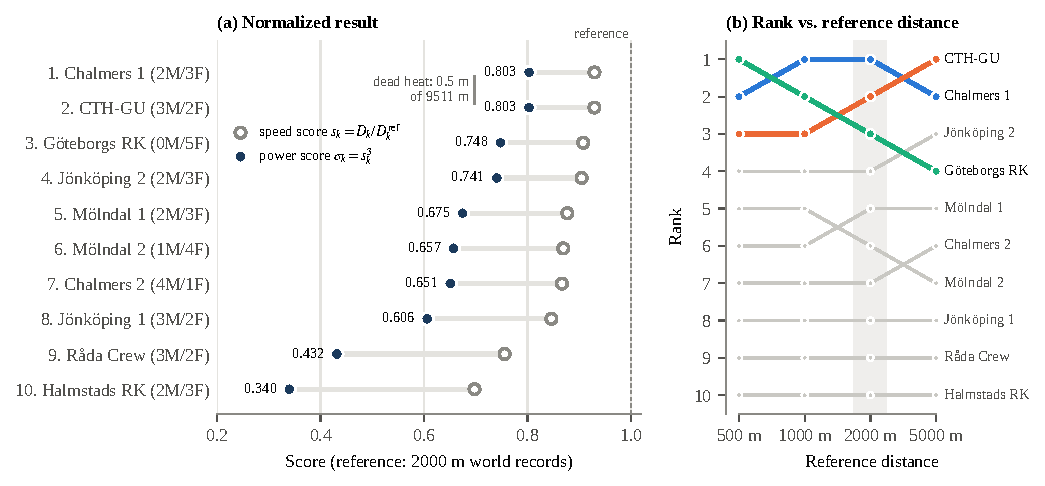
\includegraphics[width=\textwidth]{figures/results.pdf}
  \caption{(a)~Normalized result with the \SI{2000}{m} reference: power score
    $\sigma_k$ (filled) and speed score $s_k$ (open), connected per team.
    The power score shows the distance to the reference on the scale of
    produced power.
    The top two teams are separated by \TieMargin\,m.
    (b)~Rank of each team for the four reference distances of
    Table~\ref{tab:records}; the shaded column is the reference used in~(a).
    First place changes between the top three teams; positions 8--10 do not
    change.}
  \label{fig:results}
\end{figure*}

\subsection{Sensitivity to the reference distance}
\label{sec:sensitivity}

Table~\ref{tab:sensitivity} and Fig.~\ref{fig:results}b repeat the analysis
for every reference distance.
Positions 8--10 are unaffected, and positions 4--7 change by at most two
places.
First place, however, depends on the reference.
With the \SI{500}{m} records ($P_m/P_f=\RatioFive$) the all-female
G{\"o}teborgs Roddklubb wins.
With \SI{1000}{m} or \SI{2000}{m}, Chalmers Roddklubb -- Team~1 wins.
With \SI{5000}{m} ($P_m/P_f=\RatioFiveK$), CTH-GU wins.
Given how close the top three are, organizers should fix and announce the
reference before the event.
For an interval-style relay the physiologically most appropriate reference is
arguably shorter than \SI{2000}{m} (Sec.~\ref{sec:refdistance}).

\begin{table}[t]
  \centering
  \caption{Rank of each team as a function of the reference distance
    (Table~\ref{tab:records}).
    Teams are ordered by their rank with the \SI{2000}{m} reference.}
  \label{tab:sensitivity}
  \setlength{\tabcolsep}{3pt}
  \small
  \begin{tabular}{@{}lccccc@{}}
    \toprule
    Team & Comp. & 500\,m & 1000\,m & 2000\,m & 5000\,m \\
    \midrule
\tableinput{figures/sensitivity_table.tex}
    \bottomrule
  \end{tabular}
\end{table}

% ══════════════════════════════════════════════════════════════════════════════
\section{Conclusion and Outlook}

We have normalized a mixed-gender ergometer relay by the fraction $\sigma$ of
reference power sustained by each team.
Because relay members row in sequence, their distances add, and the team
reference is the power mean with exponent $1/3$ of the individual reference
powers.
The resulting score, $\sigma=(D/\Dref)^3$, needs only distances and times.
The arithmetic mean of reference powers, correct for rowers pulling together
in one boat, is biased against mixed relay teams when compared with the
power at the team's mean speed.

Expressing the score in power rather than speed does not change the order,
but reports performance on the scale the athletes actually produce, where a
few percent in speed is two to three times that in output.
What does change the order is the men-to-women reference ratio, set by the
choice of reference distance.
For RRC~2026 the leading positions are sensitive to it, and with the
\SI{2000}{m} records the top two teams are in a dead heat.

The method is implemented in the open-source Python package
\texttt{ergrace}~\cite{ergrace}, which also generates every number, table and
figure in this report.
It extends directly to age- and weight-graded references, including the
masters handicap categories of World Rowing~\cite{WorldRowingClasses}, by
replacing $P_m$ and $P_f$ with category-specific values in
Eq.~\eqref{eq:pref}.

% ──────────────────────────────────────────────────────────────────────────────
\section*{Data Availability}

The race data, normalization code, figure scripts and the source of this
report are openly available in the \texttt{ergrace} repository~\cite{ergrace}.

\section*{Acknowledgements}

The authors thank all members of M{\"o}lndals Roddklubb for their support
during the R{\aa}da Rowing Challenge.
The authors also thank Henning G.A.\ Kirchberg and Thomas Gispert for
fruitful discussions and constructive feedback on the manuscript.

\section*{Author Contributions}

LJS wrote the paper and developed the power normalization.
JL assisted with data acquisition and analysis.
OG acquired the data and supervised the project.

% ──────────────────────────────────────────────────────────────────────────────
\begin{thebibliography}{9}

\bibitem{MRKhomepage}
  M{\"o}lndals Roddklubb, \url{https://www.mrk.nu/}, accessed March 2026.

\bibitem{MRKweb2026}
  M{\"o}lndals Roddklubb, ``R{\aa}da Rowing Challenge -- 7 mars 2026,''
  \url{https://www.mrk.nu/rada-rowing-challlenge-7-mars-2026/},
  accessed March 2026.

\bibitem{Concept2manual}
  Concept2, ``RowErg Performance Monitor -- pace/power calculator,''
  \url{https://www.concept2.com/indoor-rowers/training/calculators},
  accessed March 2026.

\bibitem{Concept2records}
  Concept2, ``World Records,''
  \url{https://www.concept2.com/indoor-rowers/racing/records/world},
  accessed March 2026.

\bibitem{WorldRowingWRVIC2026}
  World Rowing, ``Records fall and champions crowned during 2026 World Rowing
  Virtual Indoor Championships, presented by Concept2,''
  \url{https://worldrowing.com/2026/02/28/records-fall-and-champions-crowned-during-2026-world-rowing-virtual-indoor-championships-presented-by-concept2/},
  28 February 2026.

\bibitem{Boyas2006}
  S.\ Boyas, A.\ Nordez, C.\ Cornu, and A.\ Gu{\'e}vel,
  ``Power responses of a rowing ergometer: mechanical sensors vs.\
  Concept2\textregistered{} measurement system,''
  \textit{Int.\ J.\ Sports Med.}\ \textbf{27}, 830--833 (2006),
  doi:10.1055/s-2006-923774.

\bibitem{WorldRowingClasses}
  World Rowing, ``Rowing Events and Boat Classes,''
  \url{https://worldrowing.com/rowing/events-boat-classes/},
  accessed March 2026.

\bibitem{ergrace}
  L.\ J.\ Splitthoff, \textit{ergrace}: ERG power normalizer for rowing relay
  competitions, \url{https://github.com/lukassplitthoff/ergrace-normalizer}, 2026.

\end{thebibliography}

\end{document}
